\section{The Large Hadron Collider}
\label{sec:lhc}

The LHC~\cite{Evans_2008} is a circular particle accelerator with a 27~kilometer ($\approx17$ miles)
circumference located, on average, approximately 100 meters beneath the Earth's surface. It is nominally
a proton-proton ($pp$) collider
but can also be run in heavy-ion configurations: proton-lead ($p$-Pb), lead-lead (Pb-Pb), or even
proton-gold ($p$-Au). It is designed to accelerate protons to a center-of-mass
energy of $\sqrt{s} = 14\,\TeV$.

To avoid the exorbitant costs in civil engineering and real-estate works associated with
constructing an even larger tunnel, it was decided that the LHC should be housed in the already-existing
tunnel that housed the Large Electron Positron (LEP) collider, in operation from 1989 to 2000.
LEP, a \textit{particle-antiparticle} collider, was able to take advantage of the fact that
 particle and anti-particle beams can be made to occupy the same phase space within a single ring: the same magnetic
fields could produce counter-rotating electron (negatively charged) and positron (positvely charged) beams.



\begin{figure}[!htb]
    \begin{center}
        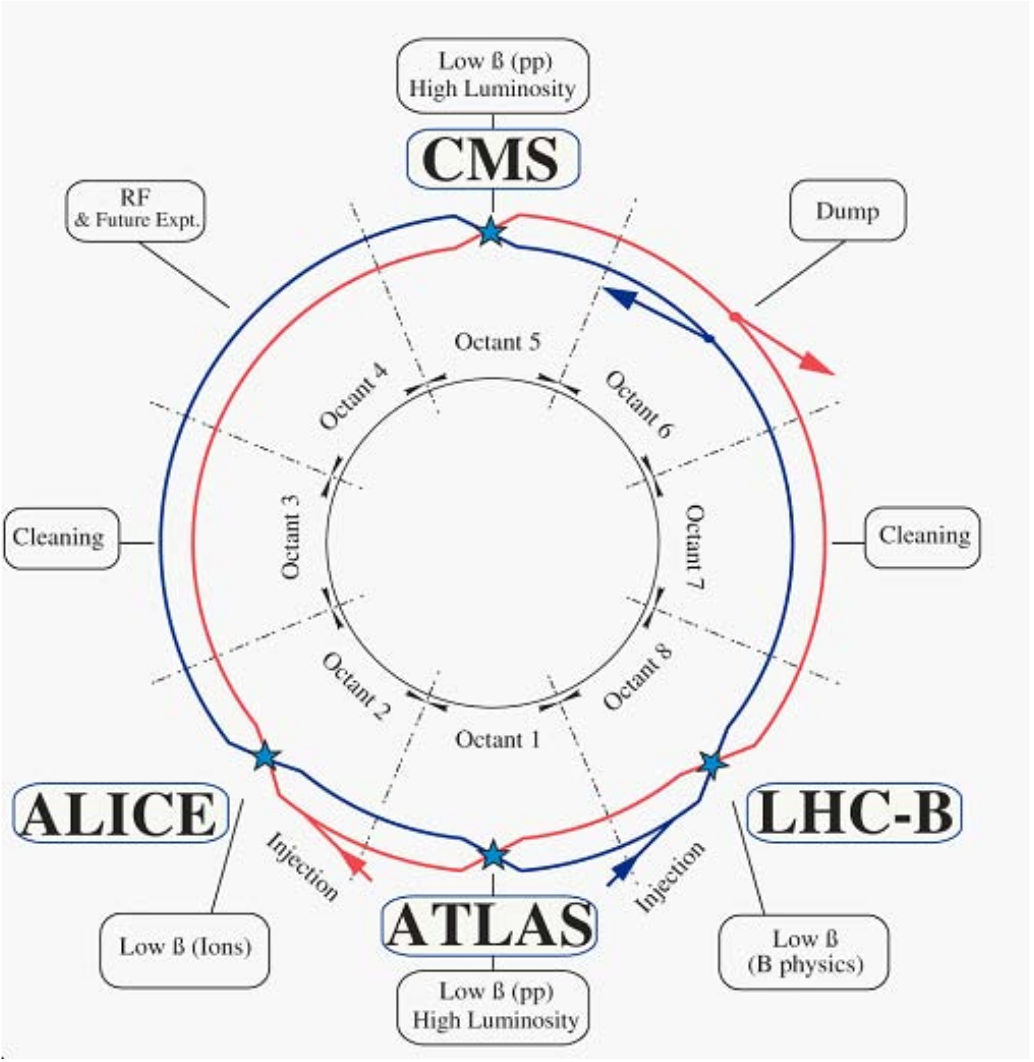
\includegraphics[width=0.8\textwidth]{figures/chapter2/lhc_layout}
        \caption{
            Layout of the LHC and its two counter-rotating beams. Beam 1 is in blue and rotates
            counter-clockwise. Beam 2 is in red and rotates clock-wise.
            At the center of each octant is a straight section which houses
            the experimental caverns or LHC beam facilities.
            At the boundaries of each octant are located the curved sections.
            Figure taken from Figure 2.1 of Ref.~\cite{Evans_2008}.
        }
        \label{fig:lhc_layout}
    \end{center}
\end{figure}

\begin{figure}[!htb]
    \begin{center}
        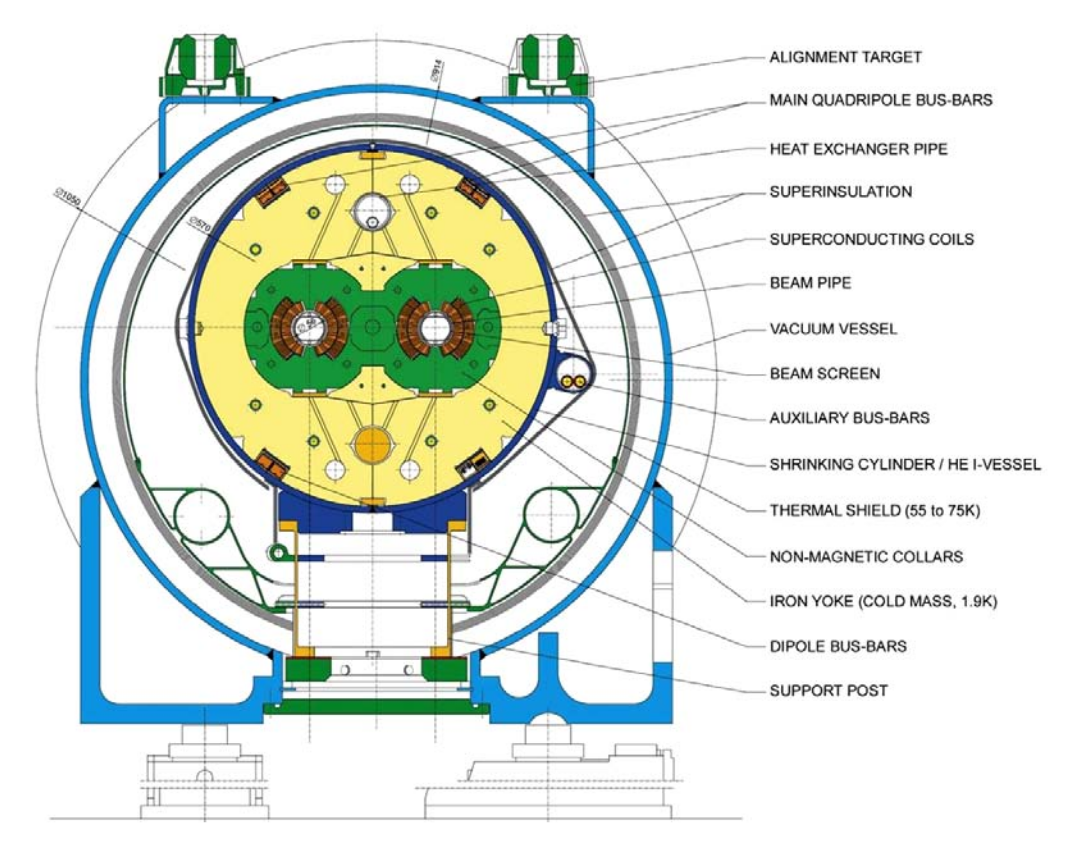
\includegraphics[width=0.5\textwidth]{figures/chapter2/lhc_dipole_fig3p3}
        \caption{
        }
        \label{fig:lhc_dipole_xsec}
    \end{center}
\end{figure}

\subsection{Injection Chain}
\label{sec:lhc_injection}

\subsection{The Concept of Luminosity}
\label{sec:lhc_luminosity}

The Large Hadron Collider (LHC) can be thought of as the final part of the particle-beam injection line
that is comprised of many parts whose goal is to accelerate protons, or other particles, to
the energies requisite for CERN's large experiments to do perform fundamental physics research
at the high-energy frontier.
